\documentclass [a4paper,12pt]{article}
\usepackage{amsmath,amsthm,amssymb}
\usepackage{graphicx}
\usepackage{mathtext}
\usepackage[T1,T2A]{fontenc}
\usepackage[utf8]{inputenc}
\usepackage[english,russian]{babel}


\title{Домашние задание №2 по дисциплине "Теория случайных процессов"}

\author{Головатских Марк \\БПМ-16-1 \\ Вариант 6}
\date{}
\begin{document}

\maketitle
\pagenumbering{gobble}
\newpage
\pagenumbering{arabic}
Обозначим за состояние $1$, когда номер телефона свободен, а за $0$, когда занят.\\
Построим граф, учитывая, что интенсивность потока, переводящего процесс из $0$ в $1$, $\mu = 4$, а из $1$ в $0$ $\lambda = 3$.\\
\begin{figure}[h!]
  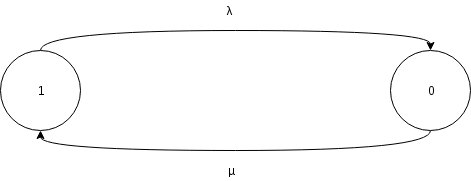
\includegraphics[width=\linewidth]{hw2.png}
\end{figure}\\
Составим уравнение Колмогорова для данного процесса:
\begin{equation*}
 \begin{cases}
  P'_1(t) = 4P_0(t) - 3P_1(t)
  \\
  P'_0(t) = 3P_1(t) - 4P_0(t)
 \end{cases}
\end{equation*}
Из записи этой системы в матричной форме получим инфинитезимальную матрицу:\\
$A = \left(
\begin{matrix}
-4 & 4\\
3 & -3\\
\end{matrix}
\right) $\\
Уравнение для нахождения распределения вероятностей для состояния $1$:\\
\begin{equation*}
 \begin{cases}
  P'_1(t) = 4 - 7P_1(t)
  \\
  P_1(0) = \frac{2}{3}
 \end{cases}
\end{equation*}
Решением является $P_1(t)=\frac{4}{7} + \frac{2}{21}e^{-7t}$.\\

Тогда вероятность, что номер свободен в момент времени $t = 2$:\\
\\$P_1(2) = \frac{4}{7} + \frac{2}{21}e^{-14} \approx 0.57142$.
\end{document}
